\documentclass[a4paper]{scrreprt}

% Uncomment to optimize for double-sided printing.
% \KOMAoptions{twoside}

% Set binding correction manually, if known.
% \KOMAoptions{BCOR=2cm}

% Localization options
\usepackage[english]{babel}
\usepackage[T1]{fontenc}
\usepackage[utf8]{inputenc}

% Quotations
\usepackage{dirtytalk}

% Floats
\usepackage{float}

\usepackage{numbertabbing}

% Enhanced verbatim sections. We're mainly interested in
% \verbatiminput though.
\usepackage{verbatim}

% Automatically remove leading whitespace in lstlisting
\usepackage{lstautogobble}

% PDF-compatible landscape mode.
% Makes PDF viewers show the page rotated by 90°.
\usepackage{pdflscape}

% Advanced tables
\usepackage{array}
\usepackage{tabularx}
\usepackage{longtable}

% Fancy tablerules
\usepackage{booktabs}

% Graphics
\usepackage{graphicx}

% Current time
\usepackage[useregional=numeric]{datetime2}

% Float barriers.
% Automatically add a FloatBarrier to each \section
\usepackage[section]{placeins}

% Custom header and footer
\usepackage{fancyhdr}

\usepackage{geometry}
\usepackage{layout}

% Math tools
\usepackage{mathtools}
% Math symbols
\usepackage{amsmath,amsfonts,amssymb}
\usepackage{amsthm}
% General symbols
\usepackage{stmaryrd}

\DeclarePairedDelimiter\abs{\lvert}{\rvert}

% Indistinguishable operator (three stacked tildes)
\newcommand*{\diffeo}{% 
  \mathrel{\vcenter{\offinterlineskip
  \hbox{$\sim$}\vskip-.35ex\hbox{$\sim$}\vskip-.35ex\hbox{$\sim$}}}}

% Bullet point
\newcommand{\tabitem}{~~\llap{\textbullet}~~}

\floatstyle{ruled}
\newfloat{algo}{htbp}{algo}
\floatname{algo}{Algorithm}
% For use in algorithms
\newcommand{\str}[1]{\textsc{#1}}
\newcommand{\var}[1]{\textit{#1}}
\newcommand{\op}[1]{\textsl{#1}}

\pagestyle{plain}
% \fancyhf{}
% \lhead{}
% \lfoot{}
% \rfoot{}
% 
% Source code & highlighting
\usepackage{listings}

% SI units
\usepackage[binary-units=true]{siunitx}
\DeclareSIUnit\cycles{cycles}

% Convenience commands
\newcommand{\mailsubject}{41106 - Cryptography Protocols - Series 3}
\newcommand{\maillink}[1]{\href{mailto:#1?subject=\mailsubject}
                               {#1}}

% Should use this command wherever the print date is mentioned.
\newcommand{\printdate}{\today}

\subject{41106 - Cryptographic Protocols}
\title{Series 3}

\author{Michael Senn \maillink{michael.senn@students.unibe.ch} - 16-126-880}

\date{\printdate}

% Needs to be the last command in the preamble, for one reason or
% another. 
\usepackage{hyperref}

\begin{document}
\maketitle


\setcounter{chapter}{2}

\chapter{Series 3}

\section{Privacy in the Google-One VPN}

Figure \ref{fig:vpn} provides an overview of a possible implementation of the
Google-One VPN described in the paper. The following algorithms elaborate on
the steps, providing additional detail where applicable.

\begin{figure}[h]
        \centering
		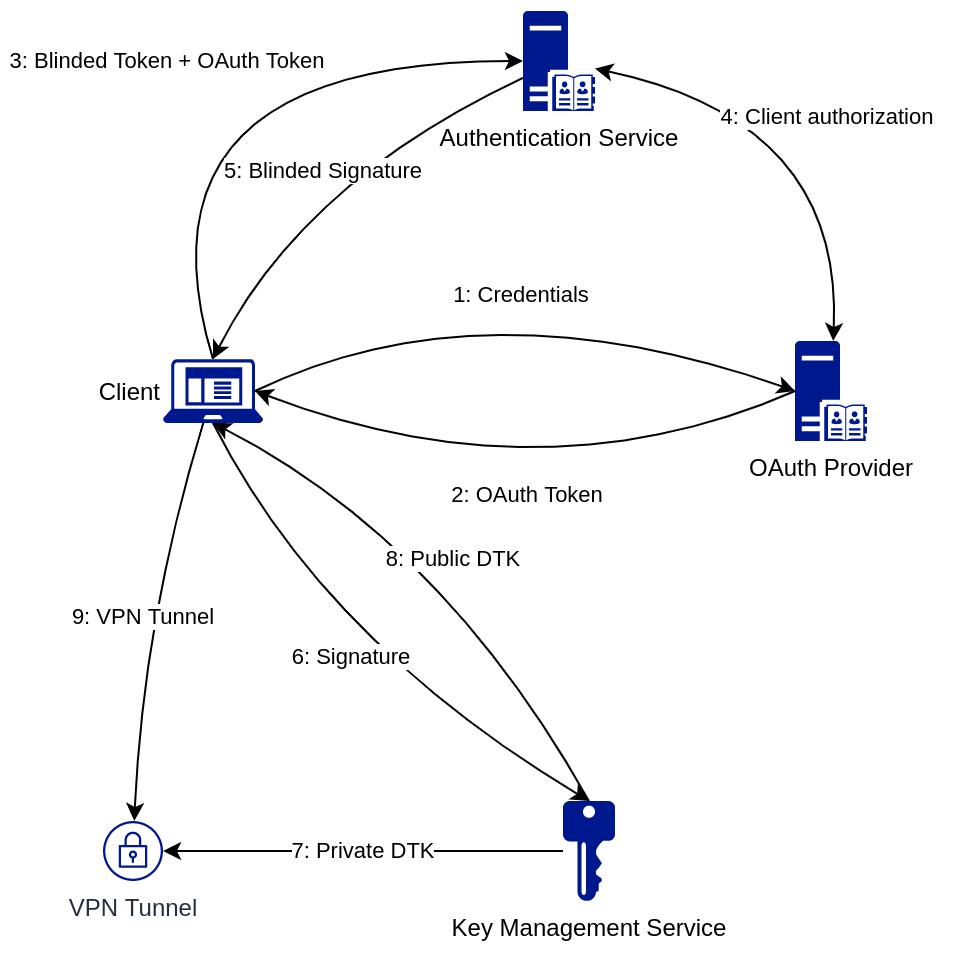
\includegraphics[width=\textwidth]{vpn}
		\caption{Google-One VPN}
		\label{fig:vpn}
\end{figure}

\subsection{Key generation \& distribution}

In a first step the authentication service will generate an RSA keypair, and
distribute the public key to the key management service and the VPN client. In
order to prevent MITM attacks this should take place via a channel providing
authenticity - e.g. by means of a public-key infrastructure.

This can, but doesn't have to, happen ahead of time. It might be perfectly
reasonable to distribute the current keypair to clients when they connect to
the authentication service, using an existing PKI for authenticity.

\begin{algo}
  \vbox{
    \small
    \begin{numbertabbing}
      xxxx\=xxxx\=xxxx\=xxxx\=xxxx\=xxxx\=MMMMMMMMMMMMMMMMMMM\=\kill
      \textbf{Authentication Service} \\
	  \> \var{((N, e), d)} := RSA.KeyGen() \\
	  \> \textbf{Send} \var{(N, e)} to \textbf{Key Management Service} and \textbf{VPN Client}
    \end{numbertabbing}
  }
  \caption{Key generation \& distribution}
  \label{alg:keygen}
\end{algo}

\FloatBarrier

\subsection{OAuth token \& blinded token generation}

The VPN client retrieves an OAuth token $T$ from the Google OAuth provider. It
then generates a random token $m$ of some length $k$ and blinds it.

\begin{algo}
  \vbox{
    \small
    \begin{numbertabbing}
      xxxx\=xxxx\=xxxx\=xxxx\=xxxx\=xxxx\=MMMMMMMMMMMMMMMMMMM\=\kill
      \textbf{VPN Client} \\
	  \> \var{T} := OAuth.authorize(credentials) \\
	  \> $m \xleftarrow{R} \{0, 1\}^k$ \\
	  \> $r \xleftarrow{R} Z_N$ \\
	  \> \var{h'} := $H(m) \cdot r^e \mod N$
    \end{numbertabbing}
  }
  \caption{OAuth token \& blinded token generation}
  \label{alg:blinded_token_generation}
\end{algo}

\FloatBarrier

\subsection{Blinded signature generation}

The VPN client sends the blinded token to the the authentication service which
checks - using the OAuth token $T$ - whether the user is authorized to use the
VPN.  If so it signs the blinded token and returns the blinded signature. The
VPN client unblinds and stores the signature.

\begin{algo}
  \vbox{
    \small
    \begin{numbertabbing}
      xxxx\=xxxx\=xxxx\=xxxx\=xxxx\=xxxx\=MMMMMMMMMMMMMMMMMMM\=\kill
      \textbf{VPN Client} \\
	  \> \textbf{Send} \var{(T, h')} to \textbf{Authentication Service}\\
	  \\
	  \textbf{Authentication Service} \\
	  \> \textbf{If} OAuth.check\_authorization(\var{T}) \\
	  \> \> \var{s'} := $h'^d \mod N$ \\
	  \> \> \textbf{Send} \var{s'} to \textbf{VPN Client} \\
	  \> \textbf{Else} \\
	  \> \> Error\\
	  \\
      \textbf{VPN Client} \\
	  \> \var{s} := $s' / r$
    \end{numbertabbing}
  }
  \caption{Blinded signature generation}
  \label{alg:signature_generation}
\end{algo}

\FloatBarrier

\subsection{VPN tunnel authentication}

The client finds a nearby VPN tunnel server $srv$ by means of $srv$. It then
sends the signature $s$, random token $m$ and server $srv$ to the key
management service. The KMS verifies whether $s$ is a valid signature for $m$.

If so a keypair to establish a secure connection with $srv$ is generated. The
private key is installed on $srv$, the public key $DTK$ sent to the client.

The client then uses $DTK$ to establish a secure VPN connection with the VPN
tunnel server. Details depend on the utilized VPN protocol, but will likely
involve deriving a shared symmetric key.

\begin{algo}
  \vbox{
    \small
    \begin{numbertabbing}
      xxxx\=xxxx\=xxxx\=xxxx\=xxxx\=xxxx\=MMMMMMMMMMMMMMMMMMM\=\kill
      \textbf{VPN Client} \\
	  \> \var{srv} := VPN.find\_nearby() \\
	  \> \textbf{Send} \var{(srv, s, m)} to \textbf{Key Management Service}\\
	  \\
	  \textbf{Key Management Service} \\
	  \> \textbf{If} $s^e = H(m)$ \\
	  \> \var{DTK} := VPN.get\_key(\var{srv}) \\
	  \> \> \textbf{Send} \var{DTk} to \textbf{VPN Client} \\
	  \> \textbf{Else} \\
	  \> \> Error\\
	  \\
      \textbf{VPN Client} \\
	  \> VPN.connect(\var{srv}, \var{DTK})
    \end{numbertabbing}
  }
  \caption{VPN tunnel authentication}
  \label{alg:vpn_authentication}
\end{algo}

\FloatBarrier

The token $m$ must be provided to prove that $s$ was issued to the client by
the authentication service, rather than being a signature the client stole from
another party. As $m$ is randomly chosen, and the authentication service only
saw the blinded token $h'$, no information about the client's identity is leaked
to the key management service in doing so.


\subsection{Key lifetime and scope}

The described architecture has a few downsides. Once a client is issued a
signature $s$ for a random token $m$ it could repeatedly use it to authenticate
itself towards the key management service. And if the VPN tunnel key $DTK$ was
static, it too could be reused by a client to authenticate itself towards the
VPN tunnel.

Both these issues can be fixed by limiting scope and lifetime of these keypairs
- with the added advantage that a potentially compromised key has less impact.

\subsubsection{RSA keypair}

The RSA keypair used by the authentication service to create signatures can be
periodically regenerated. When doing so the public key has to be redistributed
to clients and the key management service as described. This has the advantage
that any signature $s$ issued with an old keypair becomes invalid, forcing
clients to retrieve a fresh one from the authentication service.

In order to not have the signature leak information about the client's identity
it must however have a global scope, being the same (or the same set of)
keypairs for all clients.

As such this keypair has a global scope and limited lifetime.

\subsubsection{DTK}

The keypair to establish a secure tunnel connection can be specific to one
client and session. As the key management service - which generates these - has
no information about a client's identity, there is no danger in doing so.

As such these keypairs have a local scope and limited lifetime.

\end{document}
